\documentclass{article}
\usepackage{blindtext}
\usepackage[utf8]{inputenc}
\usepackage{amsmath,bm}
\usepackage{amstext}
\usepackage{amsfonts}
\usepackage{amsmath}
\usepackage{epsfig}
\usepackage{CTEX}
\usepackage[colorlinks,linkcolor=blue]{hyperref}

\title{Introduction to Machine Learning\\Homework 3}
\author{181860066 牛铭杨}

\begin{document}
	\maketitle
	\numberwithin{equation}{section}
	
	\section{[20pts] Decision Tree}

	(1) [10pts] Assume there is a space contains three binary features $X$, $Y$, $Z$ and the objective function is $f(x,y,z)=\neg(x \text{ XOR } y)$. Let $H$ denotes the decision tree constructed by these three features. Please answer the following question:
	\begin{itemize}
		\item Is function $f$ realizable? 
		\item If the answer is yes, please draw the decision tree $H$ otherwise please give the reason.\\
    \end{itemize}
    这个函数无法用决策树实现,因为决策树形成的分类边界具有轴平行的特点,分类边界由若干个和坐标轴平行的分段组成,
    对于离散属性,若已经使用这个属性划分过,之后就不能再用,所以分类边界是由折线段组成。
    而同或函数是非线性可分的,无法被一条直线分类\\\\
	(2) [10pts] Consider the following matrix:
	$$
	\left[
	\begin{matrix}
	24 & 53 & 23 & 25 & 32 & 52 & 22 & 43 & 52 & 48 \\
	40 & 52 & 25 & 77 & 48 & 110 & 38 & 44 & 27 & 65\\
	\end{matrix}
	\right]
	$$
	which contains 10 examples and each example contains two features $x_1$ and $x_2$. The corresponding label of these 10 examples as follows:
	$$
	\left[
	\begin{matrix}
	1 & 0 & 0 &1 & 1 & 1 & 1& 0 & 0 & 1
	\end{matrix}
	\right]
	$$
	In this problem, we want to build a decision tree to do the classification task.
	\begin{itemize}
		\item Calculate the entropy of the root node.
		\item Building your decision tree. What is your split rule  and the classification error?\\
	\end{itemize}

    根节点的熵为
    \begin{equation}
        {\rm Ent(D)} = -(\frac{6}{10} {\rm log_2} \frac{6}{10} + \frac{4}{10} {\rm log_2} \frac{4}{10}) = 0.971
    \end{equation}
    基于信息增益对连续属性作划分,每次选取使信息增益最大的划分属性和该属性的划分点,得到的决策树如图,该决策树的分类误差为0.\\\\
    \begin{figure}
        \centering
        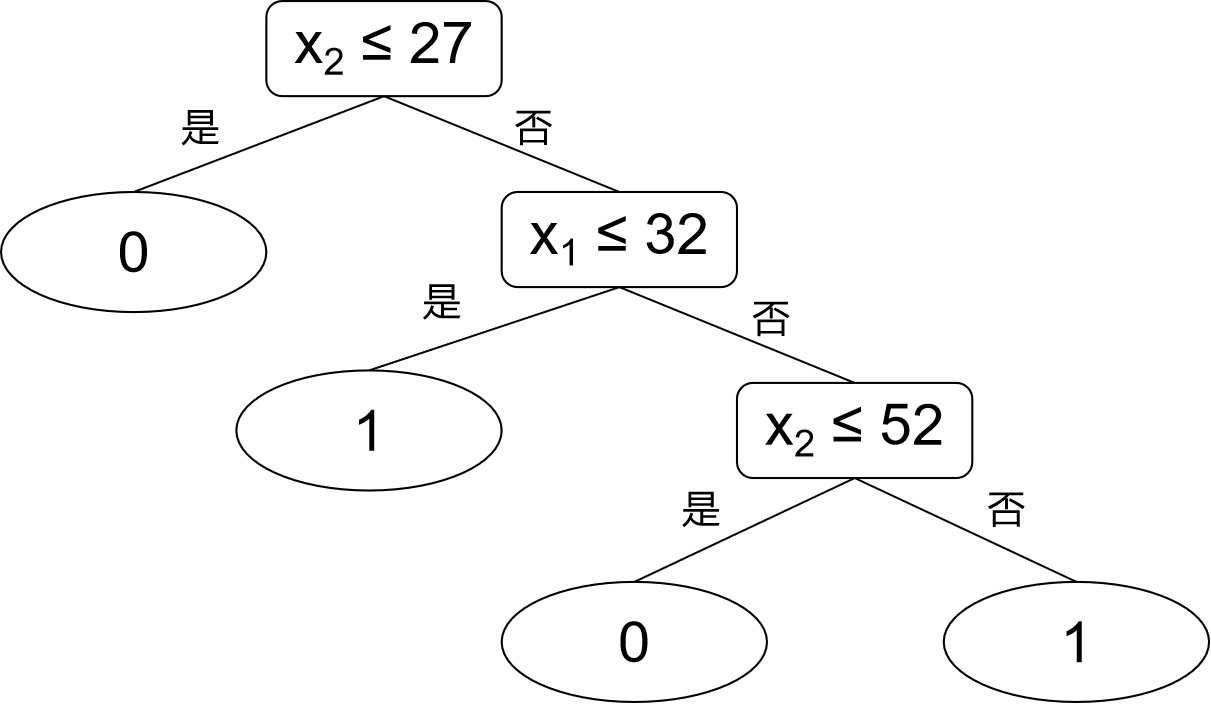
\includegraphics[width=.7\textwidth]{T1_decision_tree.png}
        \caption{决策树}
    \end{figure}
    \\\\
	\section{[20pts] Neural Network}
	Consider the following neural network, consisting of two input units, a single hidden layer containing two units, and one output unit:
	

	(1) [5pts] Assume that the network is using linear units: that is, for a given unit $U$, $A$ is the vector of activations of units that send their output to $U$ and $W$ is the weight vector corresponding to these outputs, then the output of the unit is $W^{\top}A$ Let the weight values $w_i$ be fixed, re-design the neural network to compute the same function without using any hidden units. Express the new weights in terms of the old weights.
    \\\\
    设两个隐层神经元的输出分别为$q_1$, $q_2$
    \begin{equation}
        \begin{aligned}
            q_1 &= w_1 x_1 + w_3 x_2\\
            q_2 &= w_2 x_1 + w_4 x_2\\
            y   &= w_5 q_1 + w_6 q_2\\
                &= (w_1 w_5 + w_2 w_6)x_1 + (w_3 w_5 + w_4 w_6)x_2
        \end{aligned}
    \end{equation}
    \begin{figure}
        \centering
        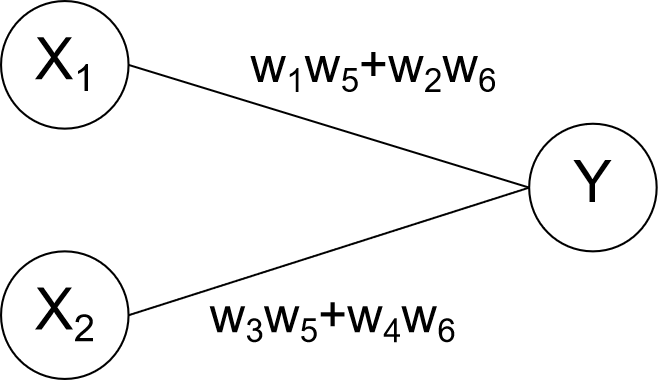
\includegraphics[width=.7\textwidth]{T2_network_without_hidden_layer.png}
        \caption{无隐层的网络}
    \end{figure}
    \\\\
	(2) [5pts] Is it always possible to express a neural network made up of only linear units without a hidden layer?
    \\\\
    总是可以。如果将神经网络架构图看成一个有向图,边的方向是从输入指向输出,那么每个$x_i$在$y$的
    最终表达式中对$y$的贡献就是$x_i$到$y$的所有路径上权值积的总和。比如在(1)中,$x_1$到$y$有两条路
    径,一条是$w_1 w_5$,另一条是$w_2 w_6$,所以$x_1$在$y$的表达式中,系数就是$w_1 w_5 + w_2 w_6$.
    所以$y$就可以看成输入$x_i$的线性组合,就可以直接将$y$与$x_i$连接,去掉隐层,每条边的权重就是
    $x_i$在$y$的表达式中的系数。
    \\\\

\end{document}
